\begin{landscape}
  \section{New Complete Amended ER Diagram for the NexStore Database}
  \begin{figure}[H]
    \centering
    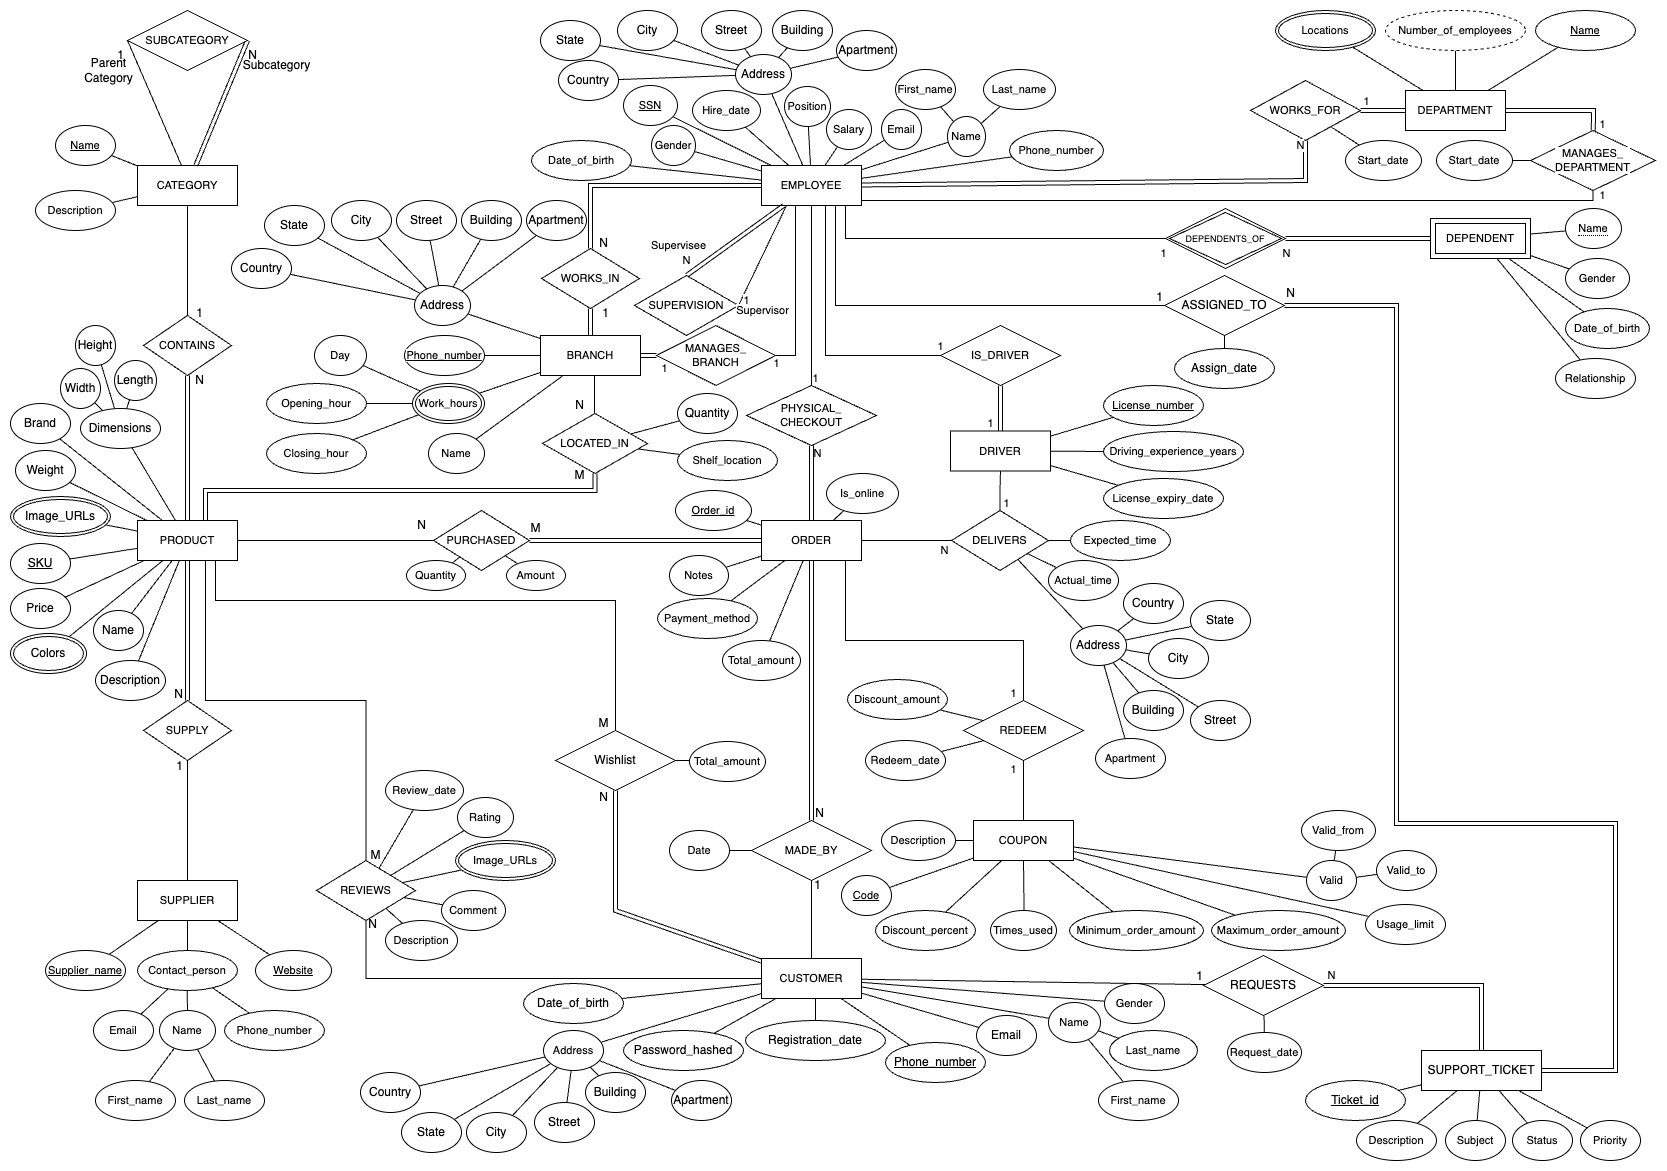
\includegraphics[width=1\textwidth]{images/diagrams/diagram.drawio.png}
    \caption{\textit{ER Diagram for the NexStore Database}}
  \end{figure}
\end{landscape}

\subsection{Entity Types and Their Attributes}

\subsubsection{Branch}
\begin{figure}[H]
  \centering
  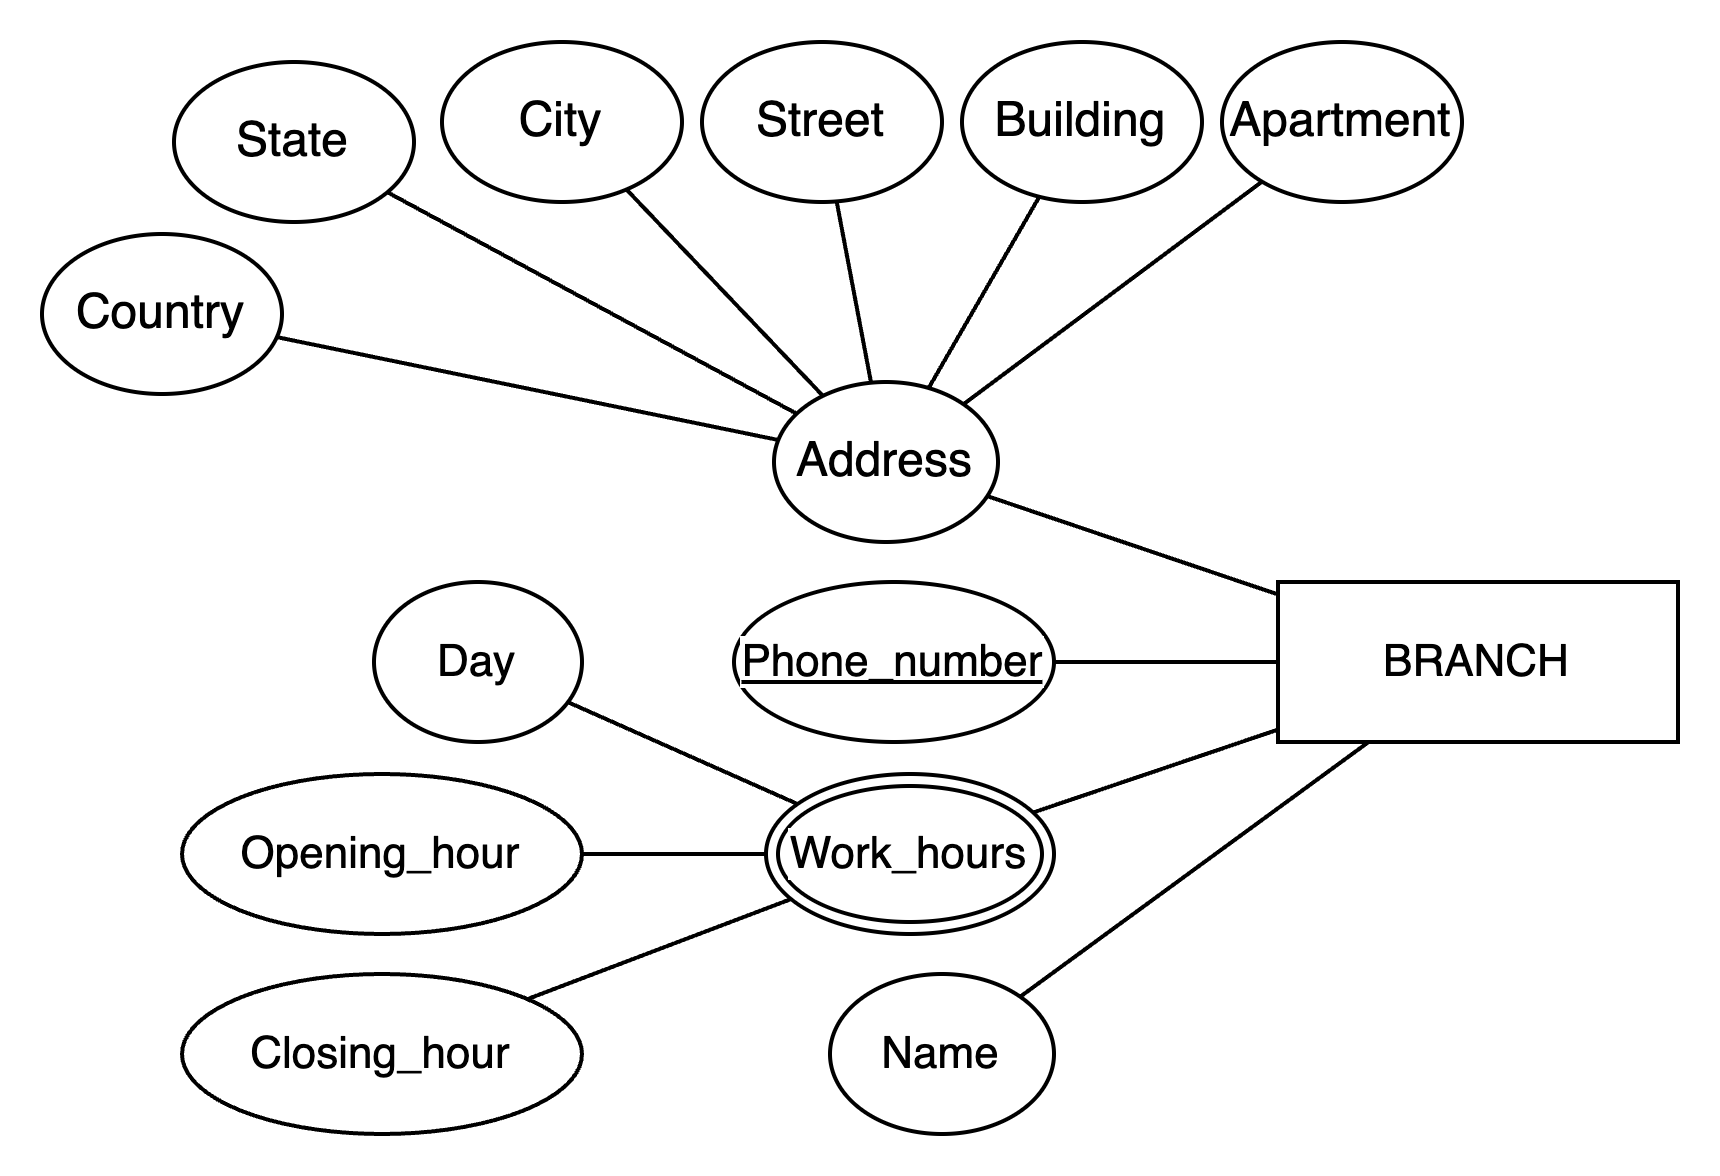
\includegraphics[width=0.7\textwidth]{images/entities/branch.png}
  \caption{\textit{Branch Entity and its Attributes}}
\end{figure}

The branch is one of the main entities presented in the ER diagram. The phone number was the primary key chosen to uniquely identify each branch. Additionally, the work hours were selected to be a composite multi-valued attribute since each branch might have different work hours depending on the weekday (e.g., weekends have different work hours). It comprises the weekday and the opening and closing hours of the branch. We included the composite attribute address to indicate the accurate address of the branch. Finally, we added the name attribute that indicates the name of each branch.

\subsubsection{Category}
\begin{figure}[H]
  \centering
  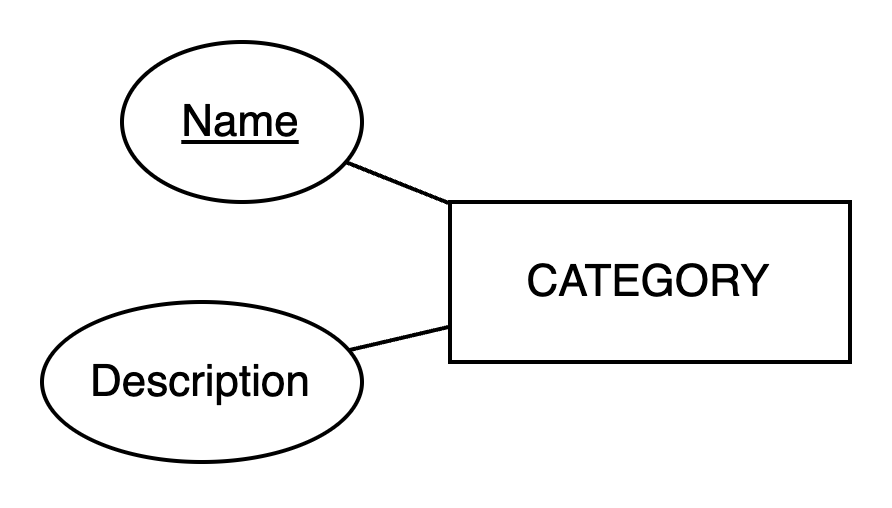
\includegraphics[width=0.6\textwidth]{images/entities/category.png}
  \caption{\textit{Category Entity and its Attributes}}
\end{figure}

As it is essential to know the category of each product, we include the category entity. It contains the Name of the category as a primary key in addition to the description of the category.

\subsubsection{Coupon}
\begin{figure}[H]
  \centering
  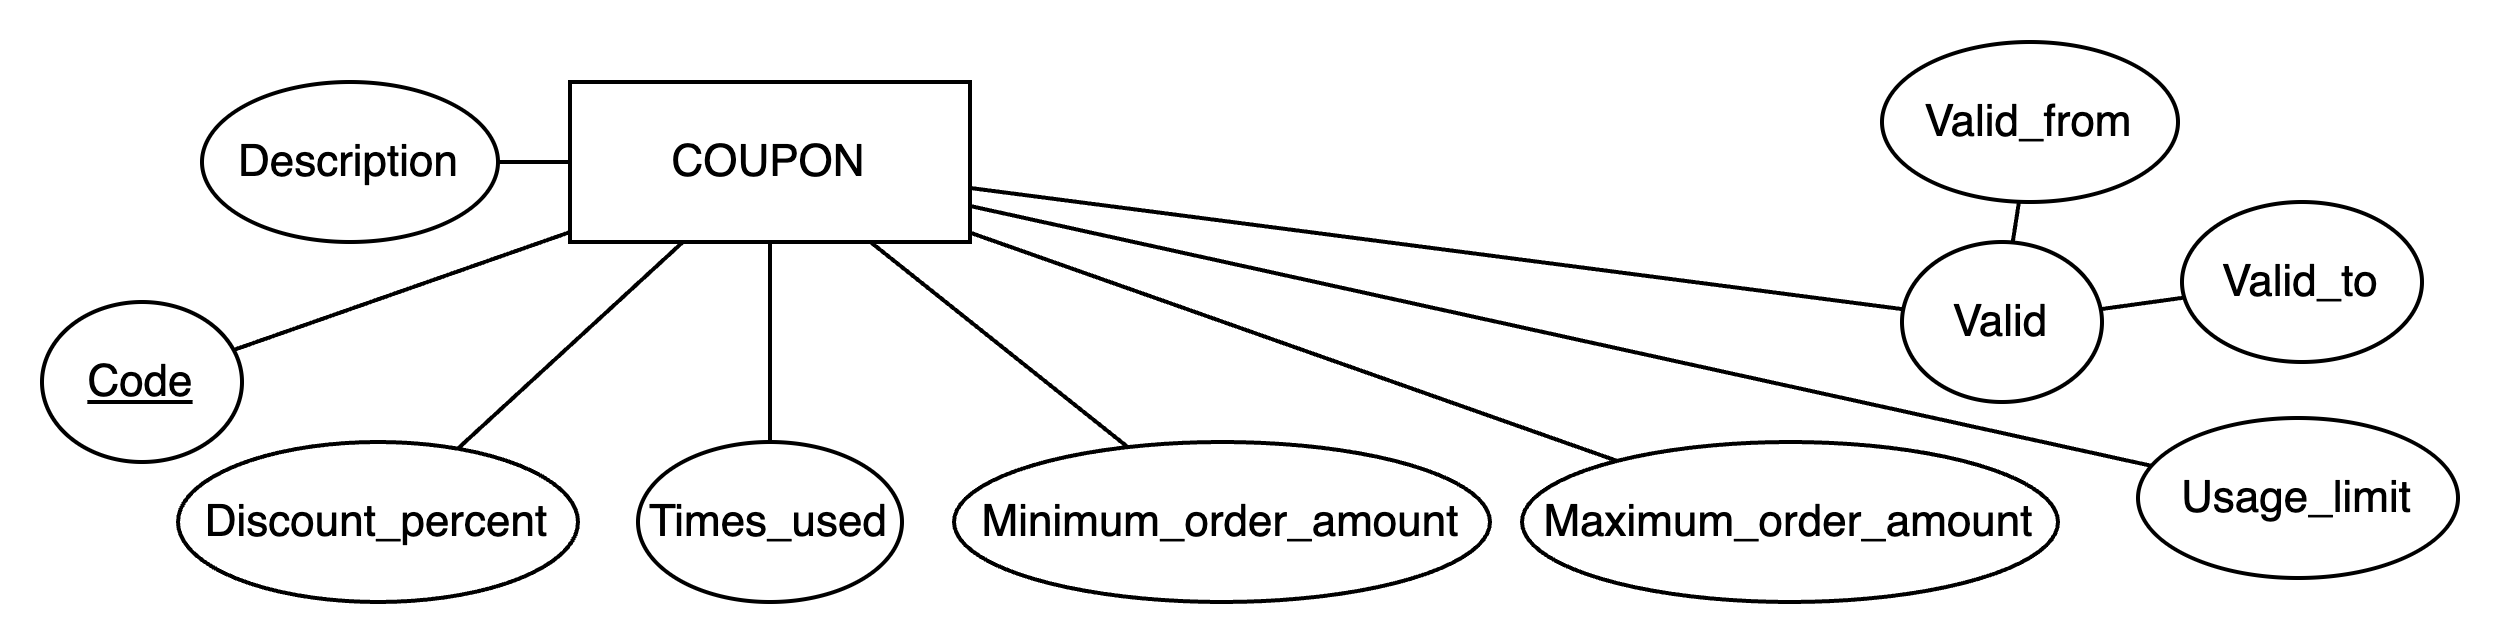
\includegraphics[width=0.7\textwidth]{images/entities/coupon.png}
  \caption{\textit{Coupon Entity and its Attributes}}
\end{figure}

In several events, a coupon might be applied to the order. The coupon can be identified by its unique code, so we chose the code to be the key attribute. Each coupon can be applied a certain number of times on a specific amount ranging from a minimum to a maximum, so we added the four attributes: "Times used", "Usage limit"," Minimum order amount" and "Maximum order amount". Furthermore, since each coupon is valid for a specific time interval, we included the "Valid to" and "Valid from" attributes. Finally, we added the attributes "Discount percent" and "Description" to indicate the discount percentage and the description of each coupon.

\subsubsection{Customer}
\begin{figure}[H]
  \centering
  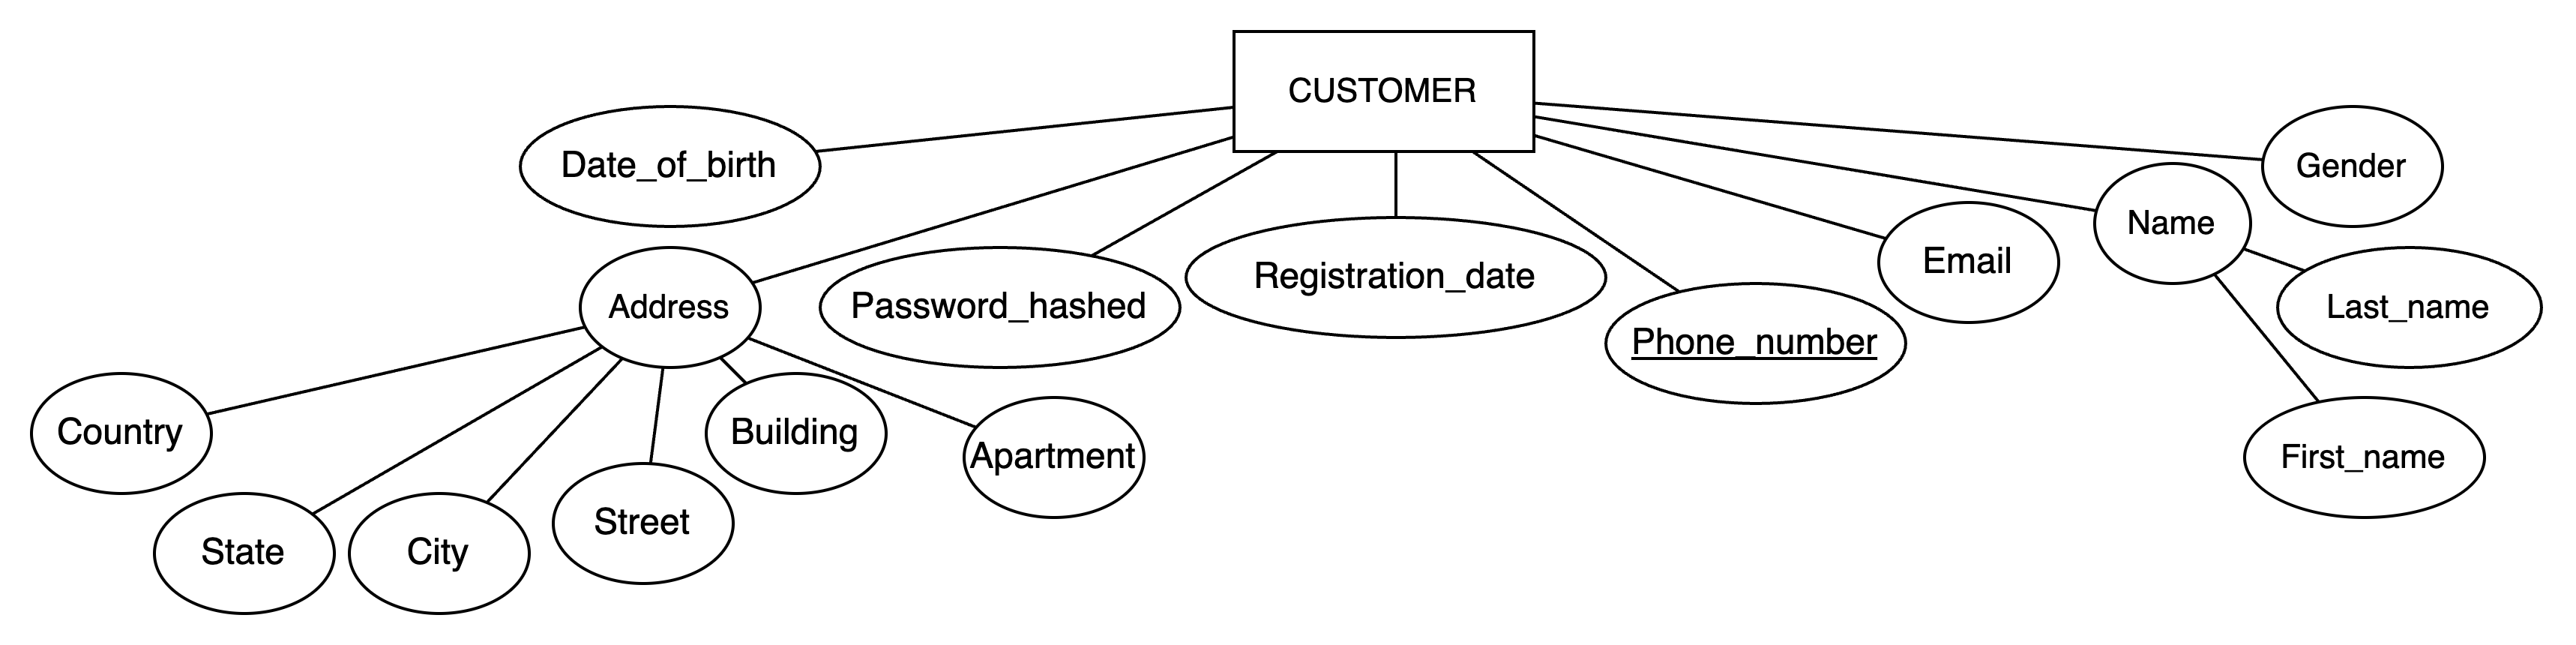
\includegraphics[width=0.7\textwidth]{images/entities/customer.png}
  \caption{\textit{Customer Entity and its Attributes}}
\end{figure}

This entity describes all the information we need to know about the customer comprising several attributes. We chose the phone number of the customer to be the primary key since it uniquely identifies each customer. Additionally, we included the name of the customer as a composite attribute as it contains the first and last name. Similarly, we added the address attribute that consists of the county, state, city, street, building, and apartment of the customer. Moreover, we added the password hashed to ensure security. Furthermore, we added the email attribute to ensure communication between the customer and the store. Finally, we added the gender, registration date, and date of birth of the customer that can be used for special events such as the customer's birthday.

\subsubsection{Department}
\begin{figure}[H]
  \centering
  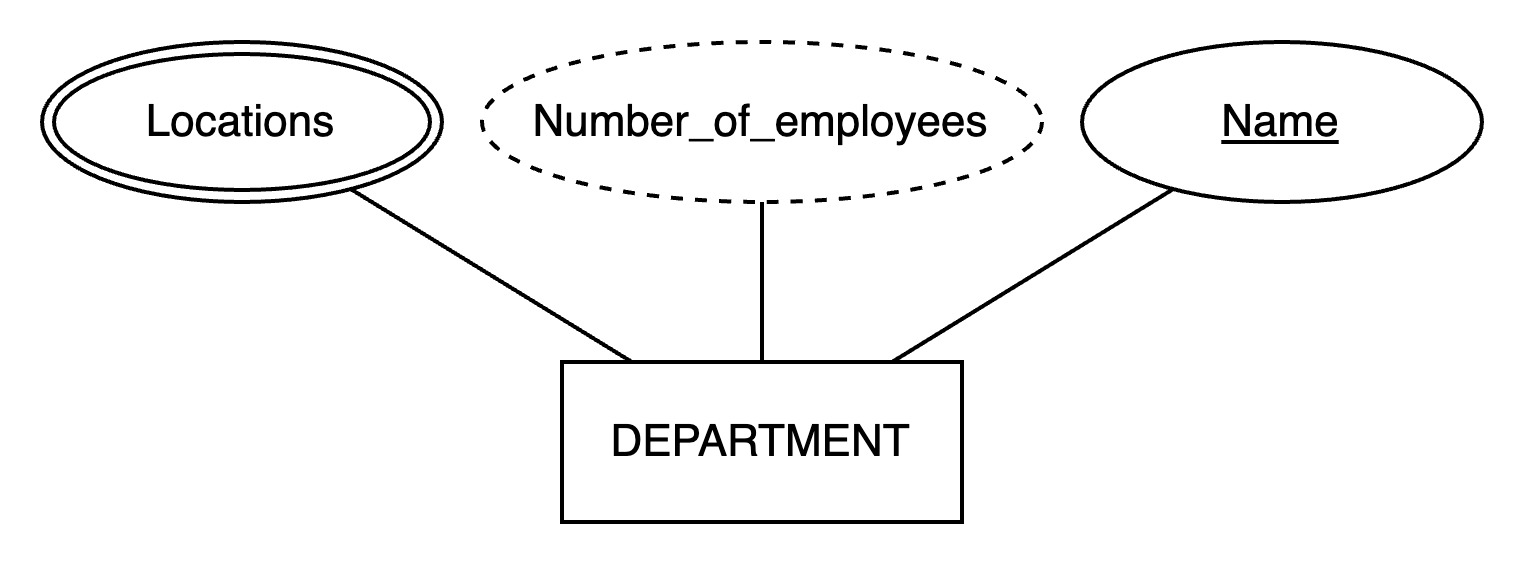
\includegraphics[width=0.7\textwidth]{images/entities/department.png}
  \caption{\textit{Department Entity and its Attributes}}
\end{figure}

This entity represents the departments in the company. Each department might have several locations, so this attribute was multi-valued. Since each department has a unique name, we chose the name to be the key attribute. Finally, we added the derived attribute "number of employees" to keep track of the updated number of employees in each department.

\subsubsection{Dependent}
\begin{figure}[H]
  \centering
  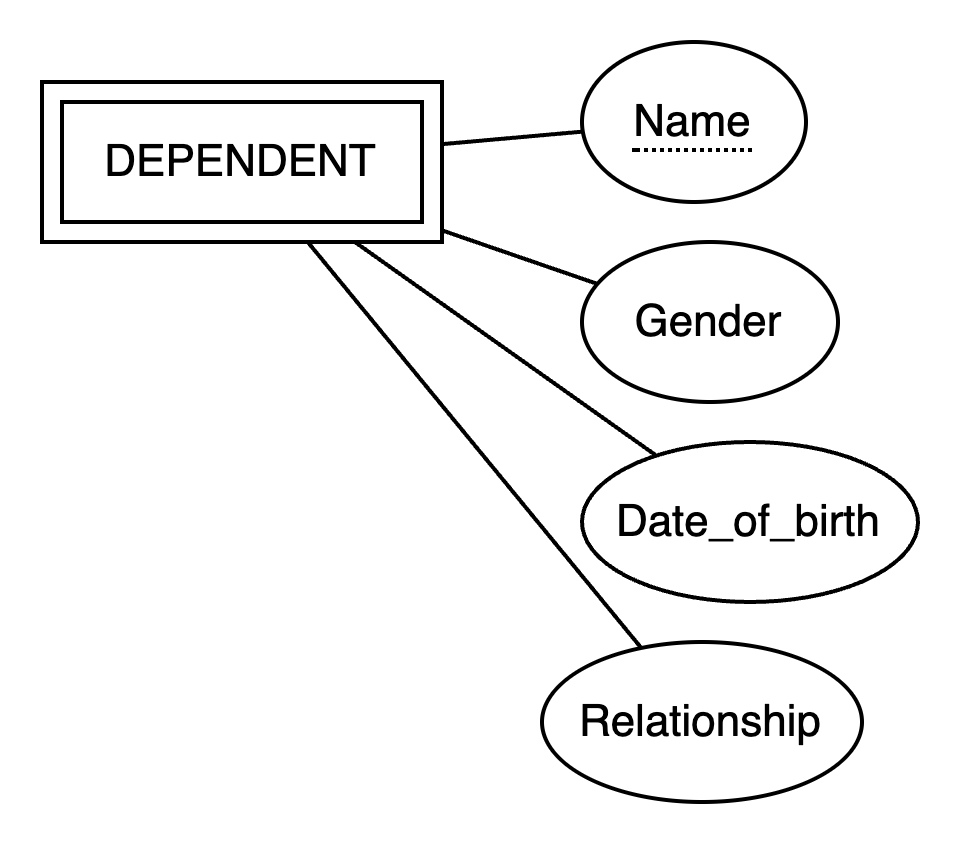
\includegraphics[width=0.7\textwidth]{images/entities/dependent.png}
  \caption{\textit{Dependent Entity and its Attributes}}
\end{figure}

Each employee has dependents that are related to them. Since we cannot have a dependent without having an employee, we set the dependent entity to be weak with the name attribute as a weak attribute of it.

\subsubsection{Driver}
\begin{figure}[H]
  \centering
  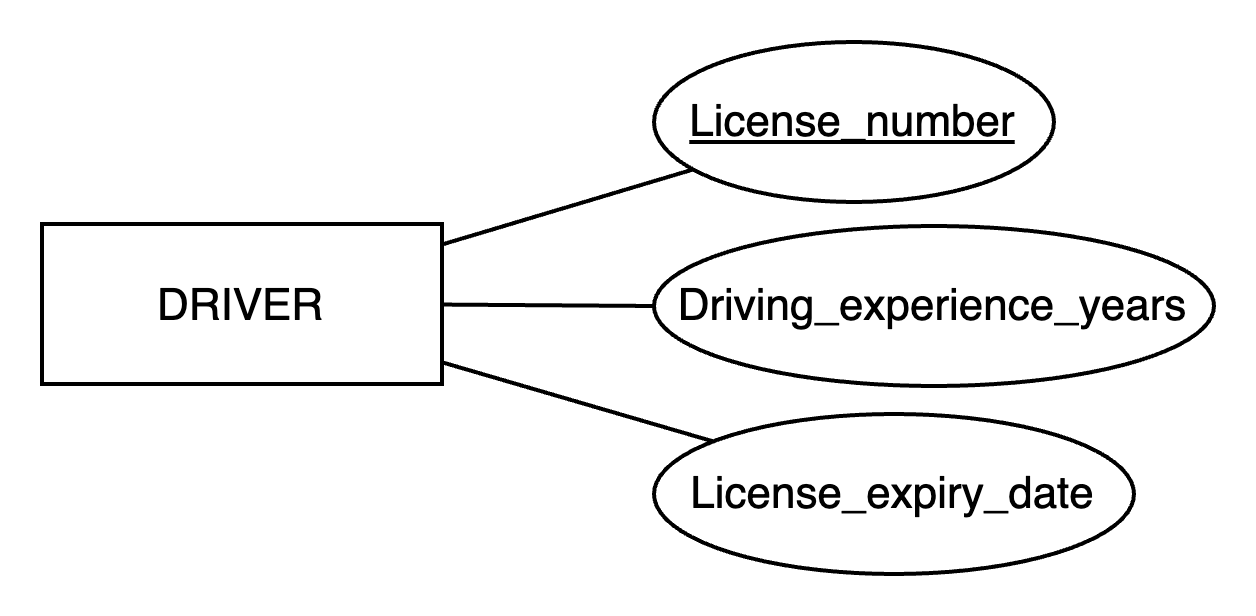
\includegraphics[width=0.7\textwidth]{images/entities/driver.png}
  \caption{\textit{Driver Entity and its Attributes}}
\end{figure}

To deliver an online order, a driver needs to be assigned. This driver entity has the license number as a primary key since it uniquely identifies the driver. Additionally, other attributes reflecting information about the driver are the driving experience years and the license expiry date.

\subsubsection{Employee}
\begin{figure}[H]
  \centering
  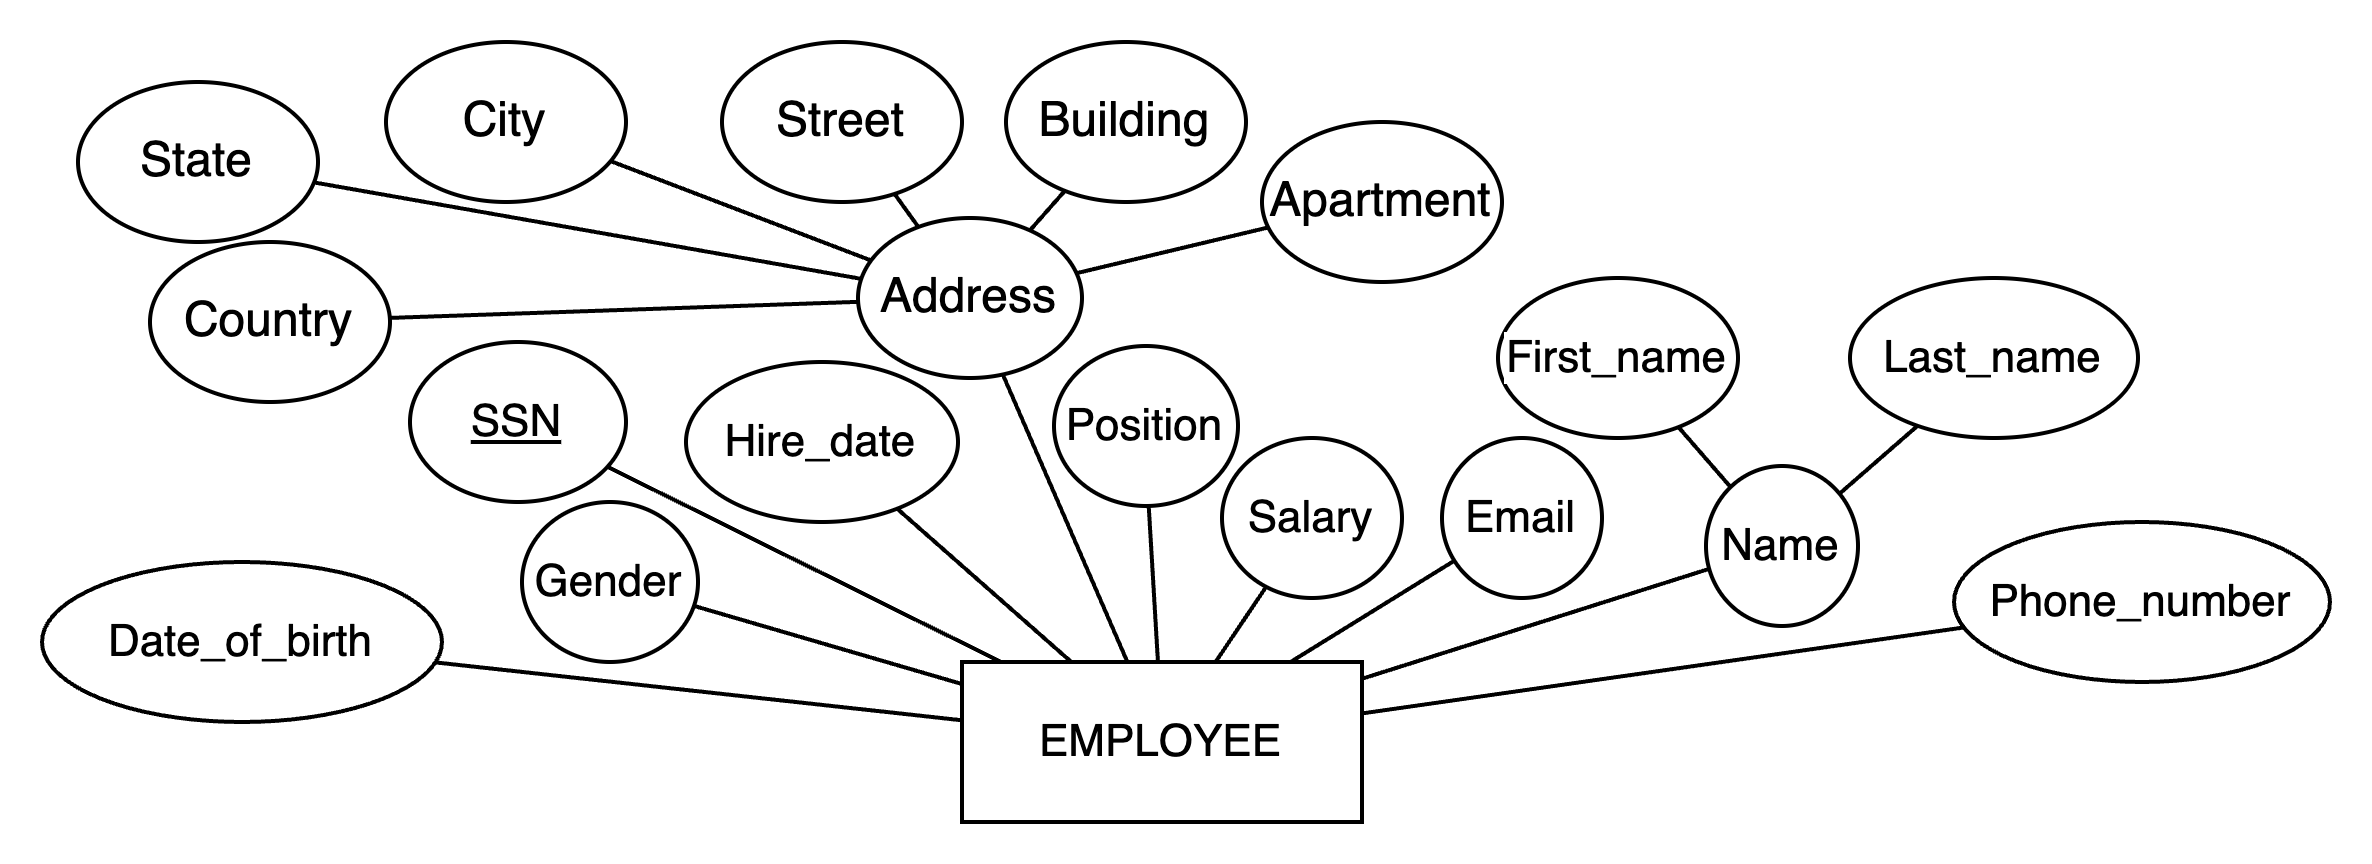
\includegraphics[width=0.7\textwidth]{images/entities/employee.png}
  \caption{\textit{Employee Entity and its Attributes}}
\end{figure}

One of the basic entities in this project is the employee entity which portrays all the information needed about the employee. We chose the social security number (SSN) of the employee as the primary key since it uniquely identifies each employee. Additionally, we added the address attribute that consists of the county, state, city, street, building, and apartment of the employee. Moreover, we included the name of the customer as a composite attribute as it contains the first and last name. Finally, we added all the information needed such as date of birth, phone number, position, gender, email address, salary, and hire date to keep an eye on this important personal information.

\subsubsection{Order}
\begin{figure}[H]
  \centering
  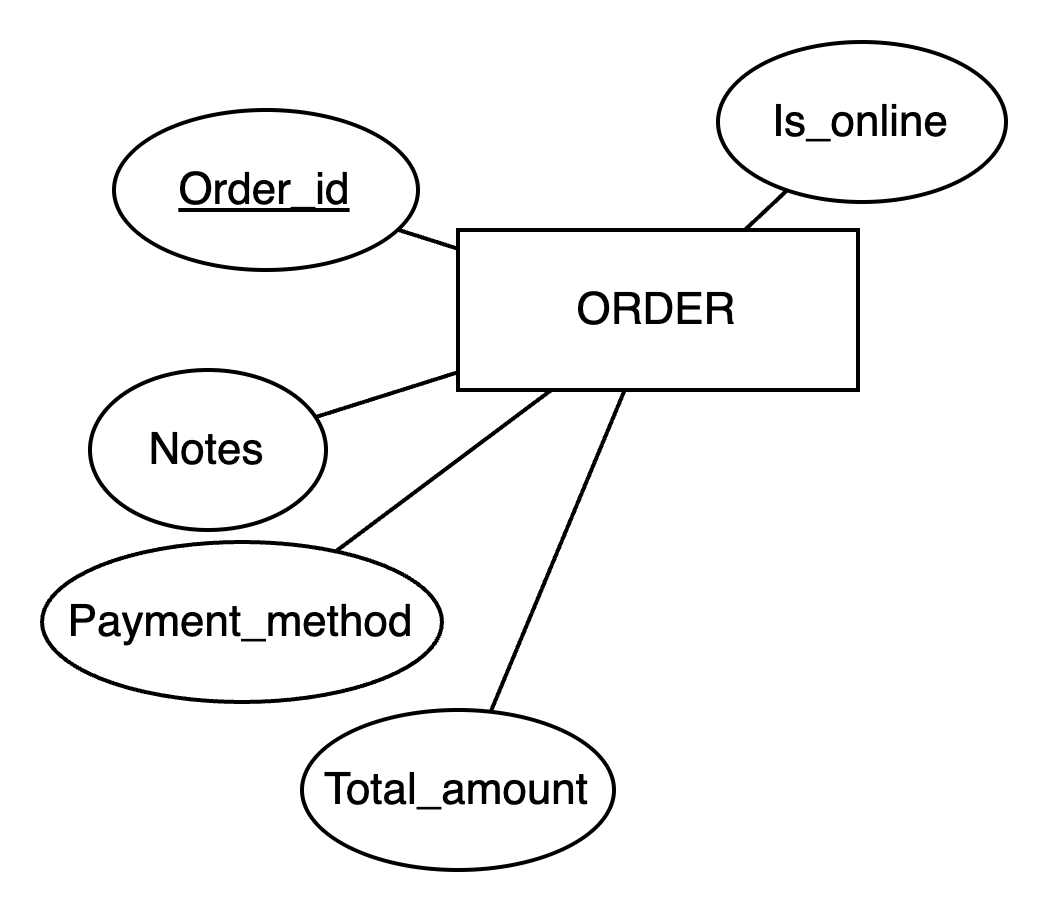
\includegraphics[width=0.7\textwidth]{images/entities/order.png}
  \caption{\textit{Order Entity and its Attributes}}
\end{figure}

To proceed with the customers' orders on both physical and online channels, the order entity was added. The primary key of this entity is the unique order ID. Other attributes include the total cost of the order, the payment method used, and any notes for this order. Finally, we added the "is online" attribute to specify whether the order was conducted physically or online.

\subsubsection{Product}
\begin{figure}[H]
  \centering
  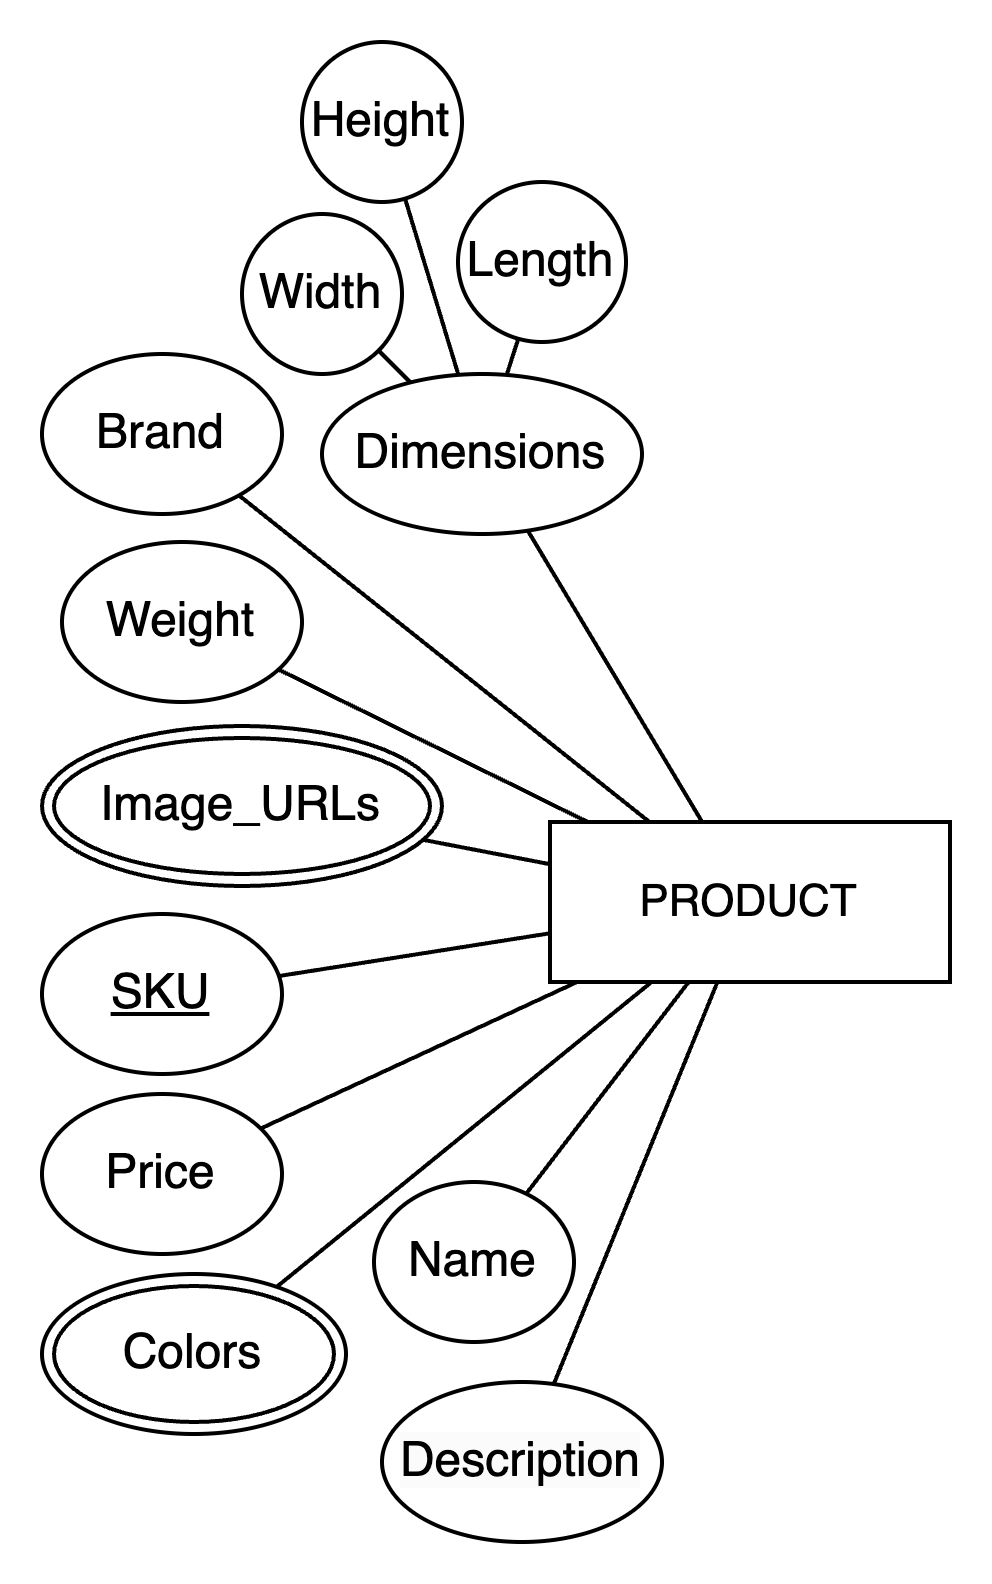
\includegraphics[width=0.7\textwidth]{images/entities/product.png}
  \caption{\textit{Product Entity and its Attributes}}
\end{figure}

This product entity describes all the information we need to know about the product comprising several attributes. We set the product entity as a weak entity since it doesn't exist without the dependence on the branch entity. We chose the stock-keeping unit (SKU) of the product as the primary key since it uniquely identifies each product. Additionally, we included the dimensions of the product as a composite attribute as it contains the height, width, and length of the product. Moreover, we added the colors as a multi-valued attribute since one product could have various colors. Similarly, we added the image URLs as a multi-valued attribute since a product could have several images to cast it online. Furthermore, we added the weight to keep track of the total weight of the shipment. In addition, we used the quantity to view the available amount of this product. Finally, we added the name, description, price, brand, and the date when the product was added to specify these essential parameters of each product.

\subsubsection{Supplier}
\begin{figure}[H]
  \centering
  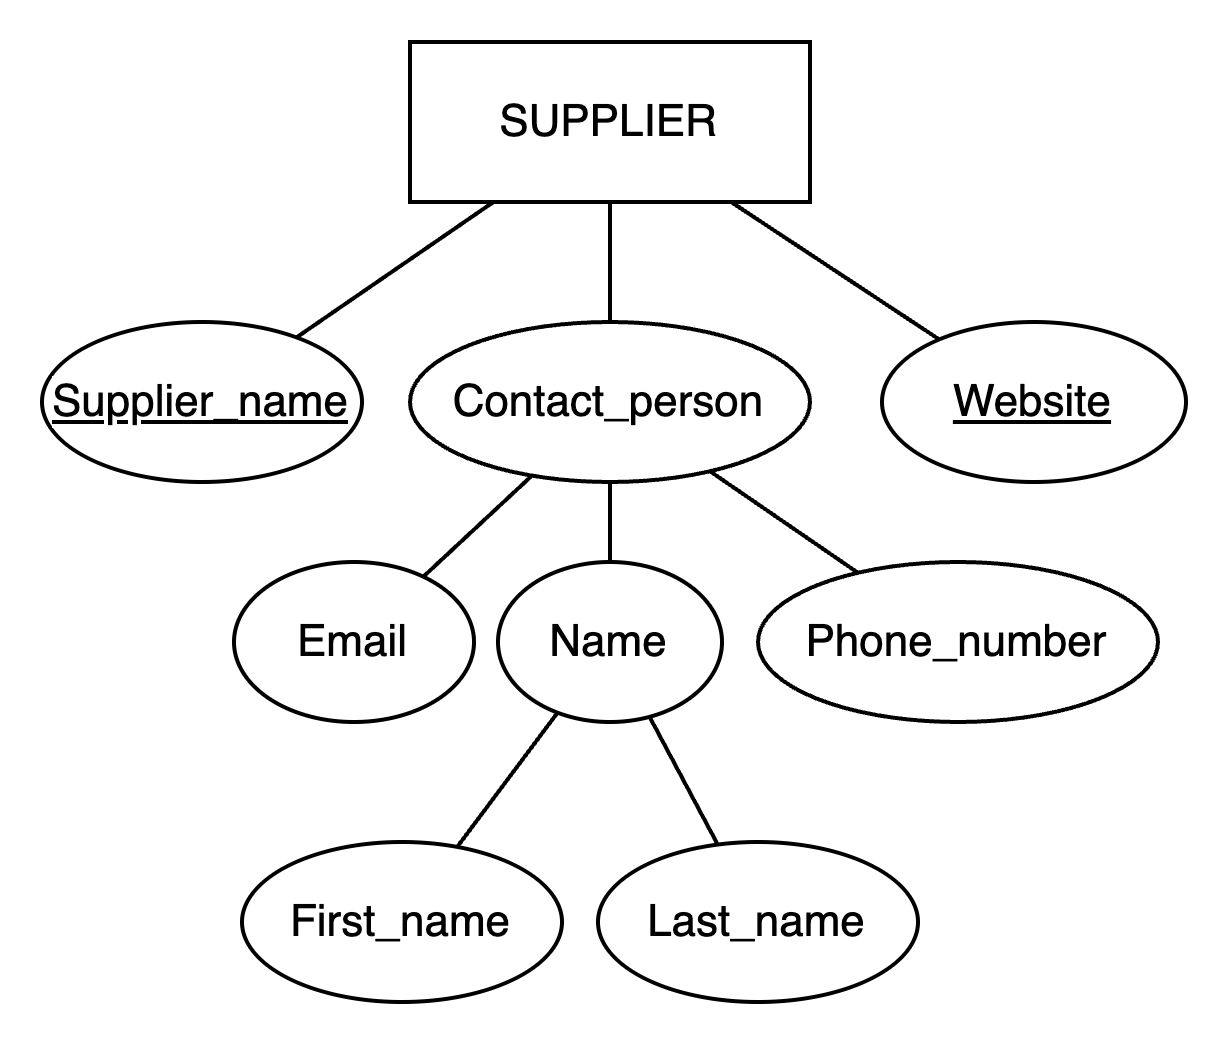
\includegraphics[width=0.7\textwidth]{images/entities/supplier.png}
  \caption{\textit{Supplier Entity and its Attributes}}
\end{figure}

Another basic entity in this project is the supplier entity which shows all the information needed about the employee. We chose the supplier's website and name as the primary keys since they uniquely identify each supplier. Finally, we included the contacted person as a composite attribute as it contains a composite attribute, the name composing the first and last name, email, and supplier's phone number.

\subsubsection{Support Ticket}
\begin{figure}[H]
  \centering
  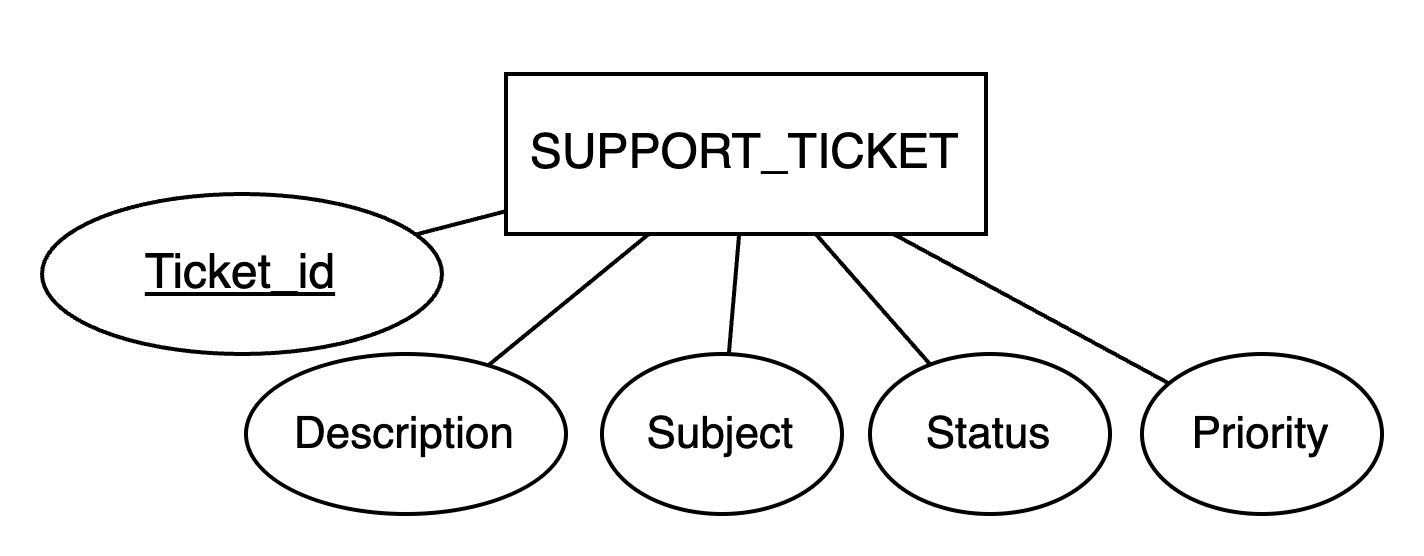
\includegraphics[width=0.7\textwidth]{images/entities/support_ticket.png}
  \caption{\textit{Support Ticket Entity and its Attributes}}
\end{figure}

To keep up with the customers' complaints, a support ticket entity was needed. We used the ticket ID as a primary key as it uniquely identifies the support ticket. Moreover, other attributes like subject, description, priority -to know how urgent the request is-, and status to keep track of it were needed.

\subsection{Relationships and their Explanations}

\subsubsection{Assigned To}
\begin{figure}[H]
  \centering
  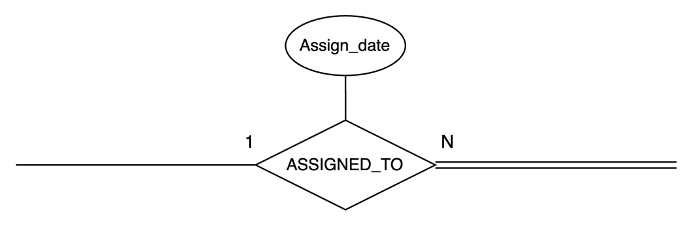
\includegraphics[width=0.7\textwidth]{images/relationships/assigned_to.png}
  \caption{\textit{Assigned To Relationship}}
\end{figure}

The relationship "assigned to" is between the employee and the support ticket. It maps the employee to zero or more support tickets and stores the data of the assignment. Also, it supports the real-life need that a support ticket must be assigned to an employee.

\subsubsection{Contains}
\begin{figure}[H]
  \centering
  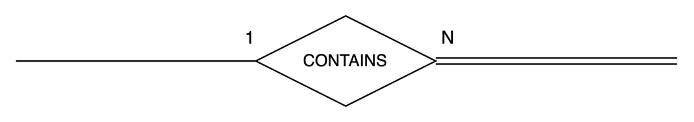
\includegraphics[width=0.7\textwidth]{images/relationships/contains.png}
  \caption{\textit{Contains Relationship}}
\end{figure}

The relationship "contains" is between a category and products. A category may contain many products. This organized the products the company has by categorizing all the products under specific categories. Also, it helps a better user experience by searching the category and then looking for the specific product needed in the category.

\subsubsection{Delivers}
\begin{figure}[H]
  \centering
  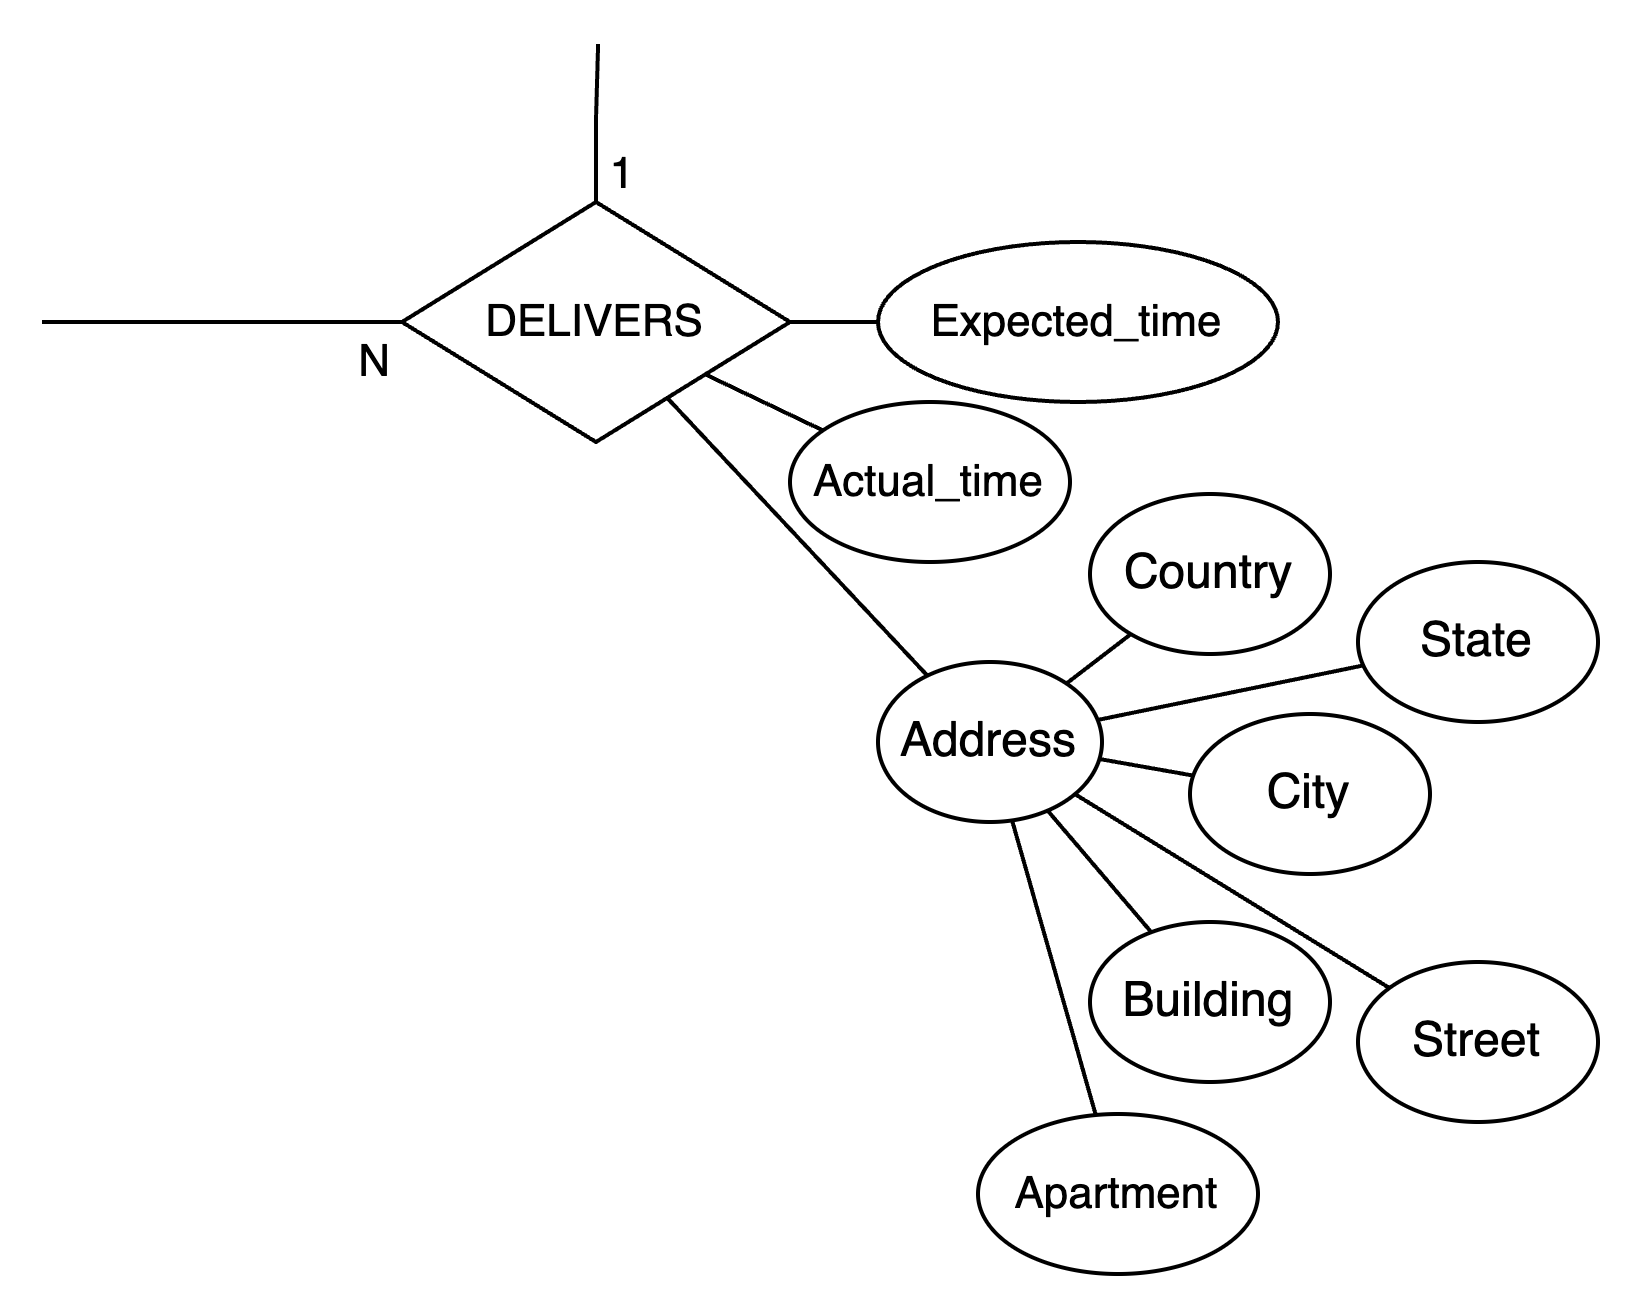
\includegraphics[width=0.7\textwidth]{images/relationships/delivers.png}
  \caption{\textit{Delivers Relationship}}
\end{figure}

The relationship "Delivers" is between the Driver and the Order. The driver is responsible for delivering the order to the requested address provided by the customer. It includes the "expected time" attribute to be displayed to the customer and the "actual time" attribute to help predict accurate delivery times for future orders. A driver can deliver many orders, but each order is delivered by one driver. Some orders may be physically checked out, in which case no delivery is required.

\subsubsection{Dependents Of}
\begin{figure}[H]
  \centering
  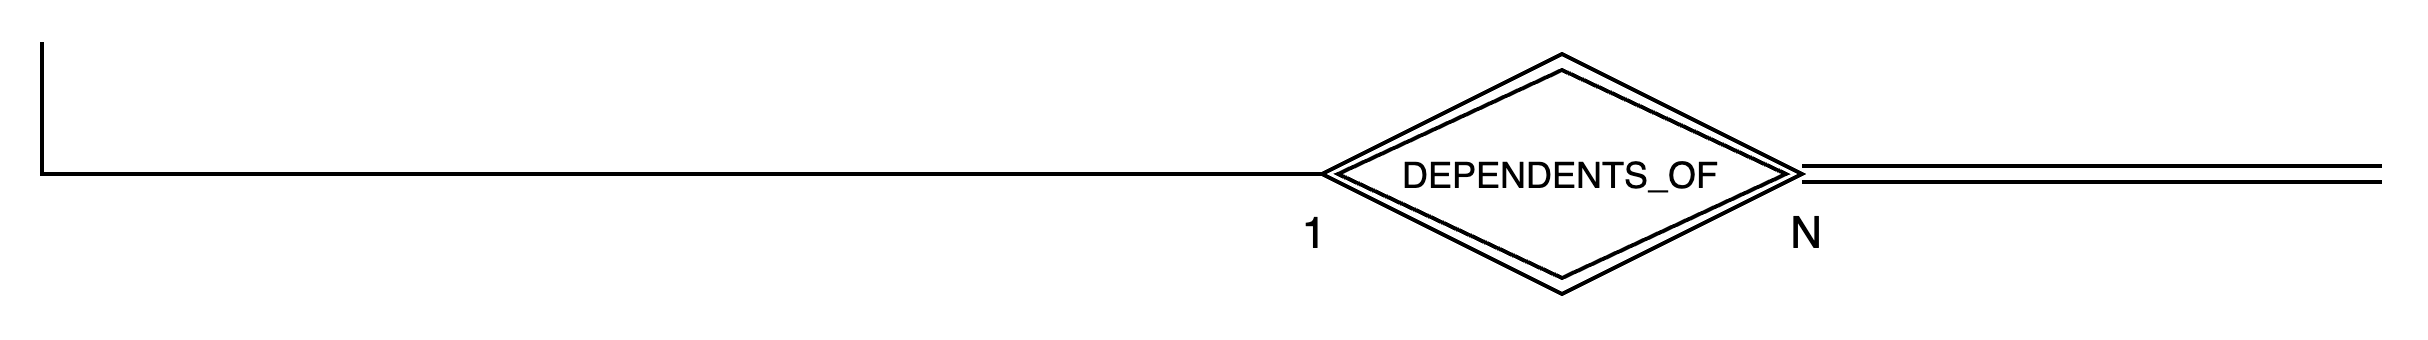
\includegraphics[width=0.7\textwidth]{images/relationships/dependents_of.png}
  \caption{\textit{Dependents Of Relationship}}
\end{figure}

The "Dependents Of" relationship is between the Employee and the Dependent. Each employee may have several dependents. This relationship is essential for connecting employees to their dependents, who might be insured by the company in the future.

\subsubsection{Is Driver}
\begin{figure}[H]
  \centering
  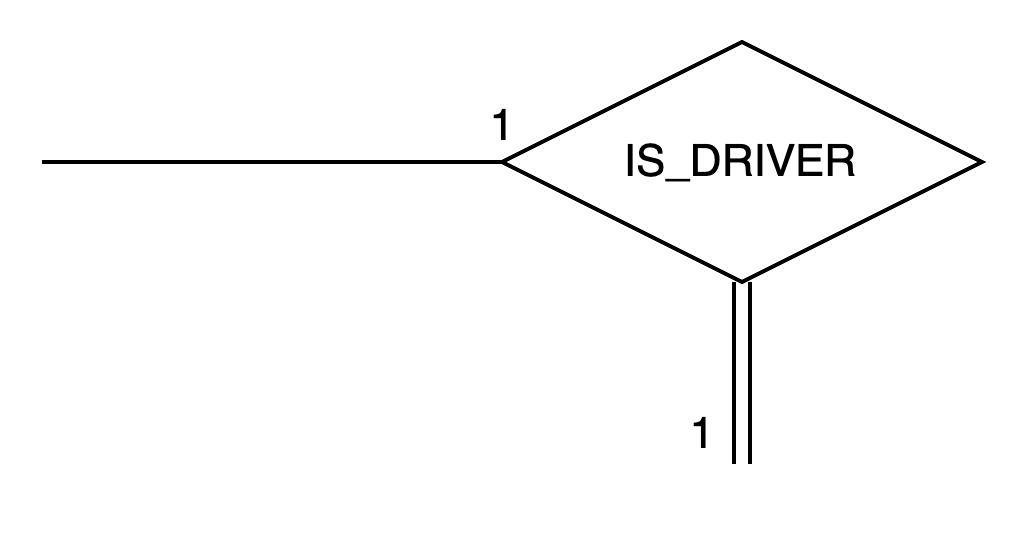
\includegraphics[width=0.7\textwidth]{images/relationships/is_driver.png}
  \caption{\textit{Is Driver Relationship}}
\end{figure}

The "Is Driver" relationship is between the Employee and the Driver. Each driver is also an employee of the company, and this relationship helps categorize employees based on whether they are drivers.

\subsubsection{Located In}
\begin{figure}[H]
  \centering
  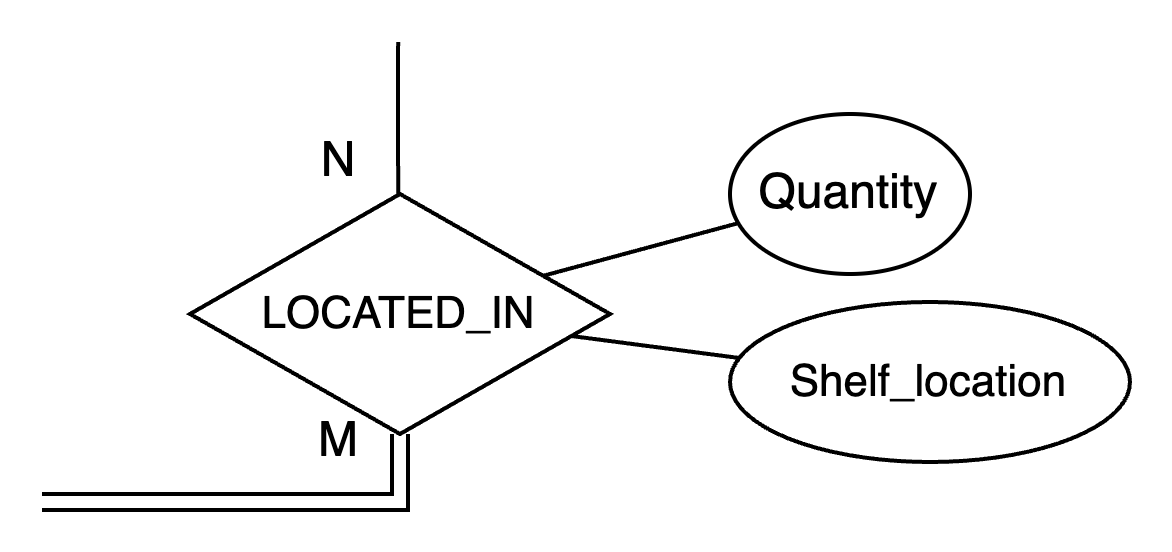
\includegraphics[width=0.7\textwidth]{images/relationships/located_in.png}
  \caption{\textit{Located In Relationship}}
\end{figure}

The "Located In" relationship is between the Product and the Branch. A branch can stock multiple products, each with specific quantities placed on certain shelves. The quantity and shelf location may vary between branches to avoid redundancy.

\subsubsection{Made By}
\begin{figure}[H]
  \centering
  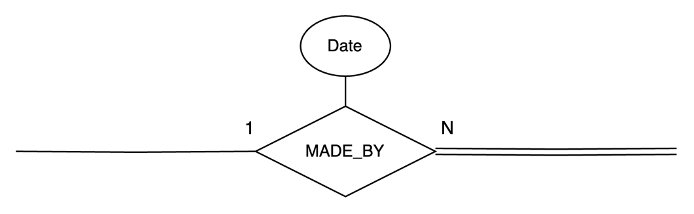
\includegraphics[width=0.7\textwidth]{images/relationships/made_by.png}
  \caption{\textit{Made By Relationship}}
\end{figure}

The "Made By" relationship connects the Customer and the Order. Each order is placed by one customer, but a customer can place multiple orders. This relationship also stores the order date for tracking purposes.

\subsubsection{Manages Branch}
\begin{figure}[H]
  \centering
  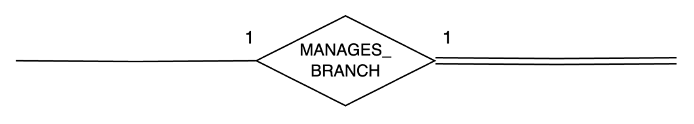
\includegraphics[width=0.7\textwidth]{images/relationships/manages_branch.png}
  \caption{\textit{Manages Branch Relationship}}
\end{figure}

The "Manages Branch" relationship is between the Employee and the Branch. Each branch is managed by one employee, but not all employees are managers. This relationship helps define the company's management structure.

\subsubsection{Manages Department}
\begin{figure}[H]
  \centering
  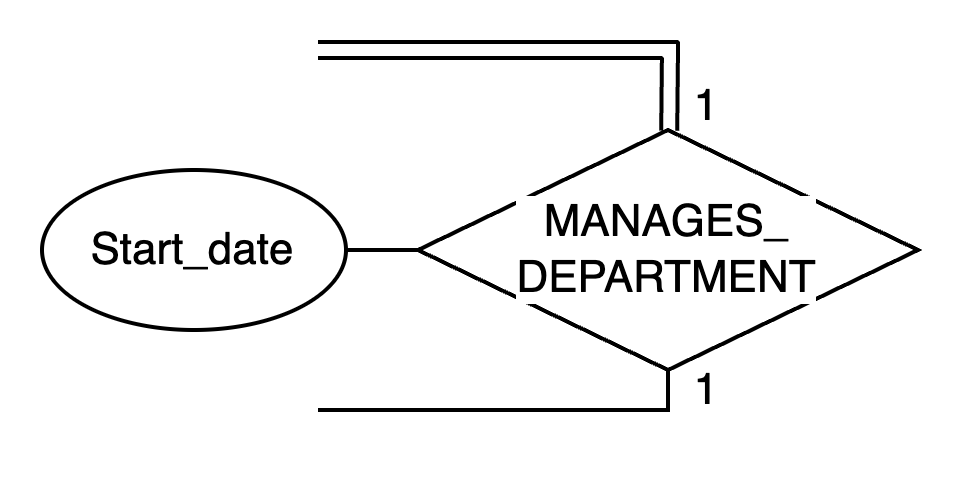
\includegraphics[width=0.7\textwidth]{images/relationships/manages_department.png}
  \caption{\textit{Manages Department Relationship}}
\end{figure}

The "Manages Department" relationship is between the Employee and the Department. An employee can manage one department, enabling a clear tracking of department managers.

\subsubsection{Physical Checkout}
\begin{figure}[H]
  \centering
  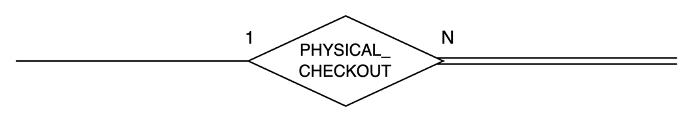
\includegraphics[width=0.7\textwidth]{images/relationships/physical_checkout.png}
  \caption{\textit{Physical Checkout Relationship}}
\end{figure}

The "Physical Checkout" relationship is between the Employee and the Order. Each order must be checked out by one employee, but an employee can check out multiple orders. This relationship prevents duplicate receipts and streamlines order management.

\subsubsection{Purchased}
\begin{figure}[H]
  \centering
  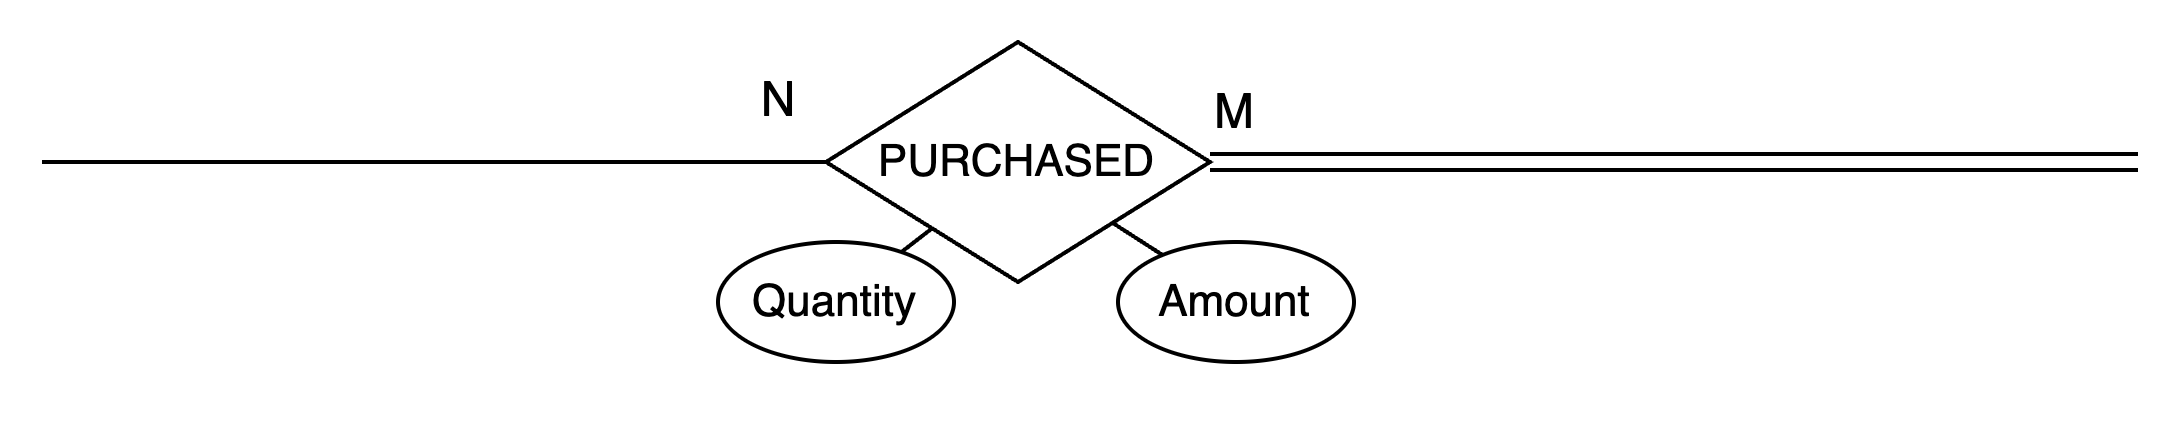
\includegraphics[width=0.7\textwidth]{images/relationships/purchased.png}
  \caption{\textit{Purchased Relationship}}
\end{figure}

The "Purchased" relationship is between the Product and the Order. An order can contain multiple products, each with specific quantities and prices. This relationship tracks these details to calculate the total order value.

\subsubsection{Redeem}
\begin{figure}[H]
  \centering
  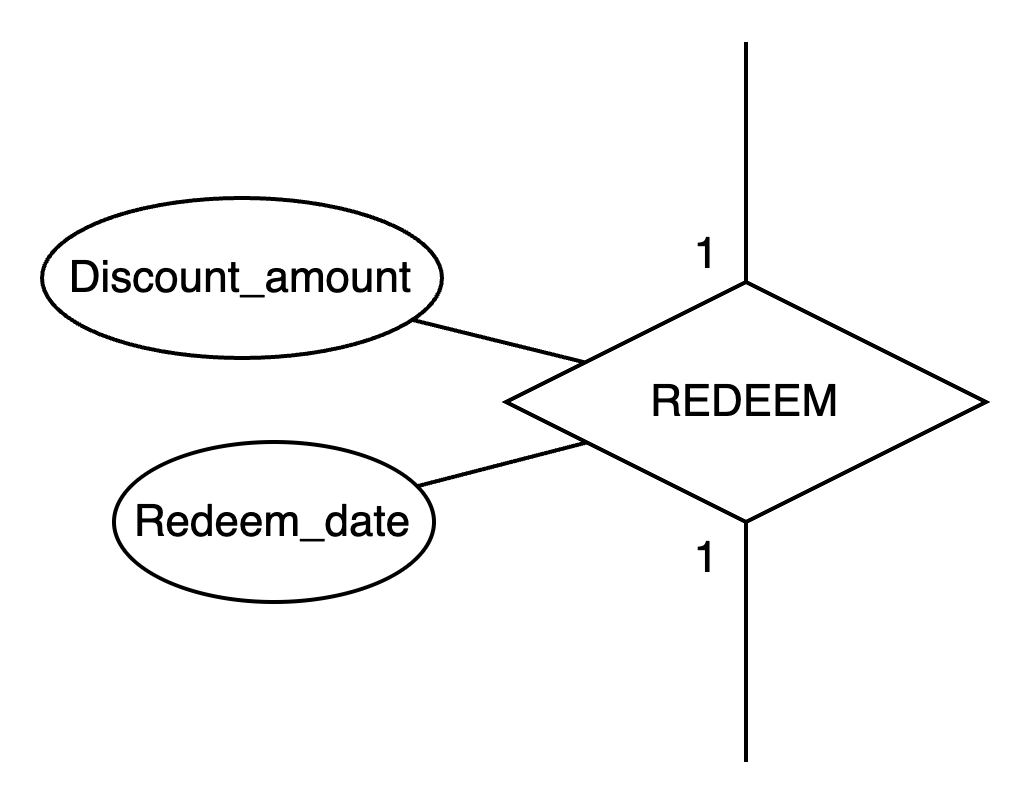
\includegraphics[width=0.6\textwidth]{images/relationships/redeem.png}
  \caption{\textit{Redeem Relationship}}
\end{figure}

The "Redeem" relationship connects the Order and the Coupon. An order can be redeemed using one coupon, and a coupon can only redeem one order. This relationship supports special occasion discounts.

\subsubsection{Request}
\begin{figure}[H]
  \centering
  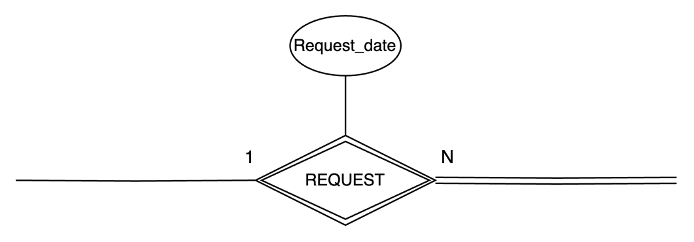
\includegraphics[width=0.7\textwidth]{images/relationships/request.png}
  \caption{\textit{Request Relationship}}
\end{figure}

This relationship is between the customer and the support ticket. It enables the customer to create various support tickets, but a ticket can't be created without the request of the customer. By including this relationship in our system, it manages the complaints of the customers efficiently.

\subsubsection{Reviews}
\begin{figure}[H]
  \centering
  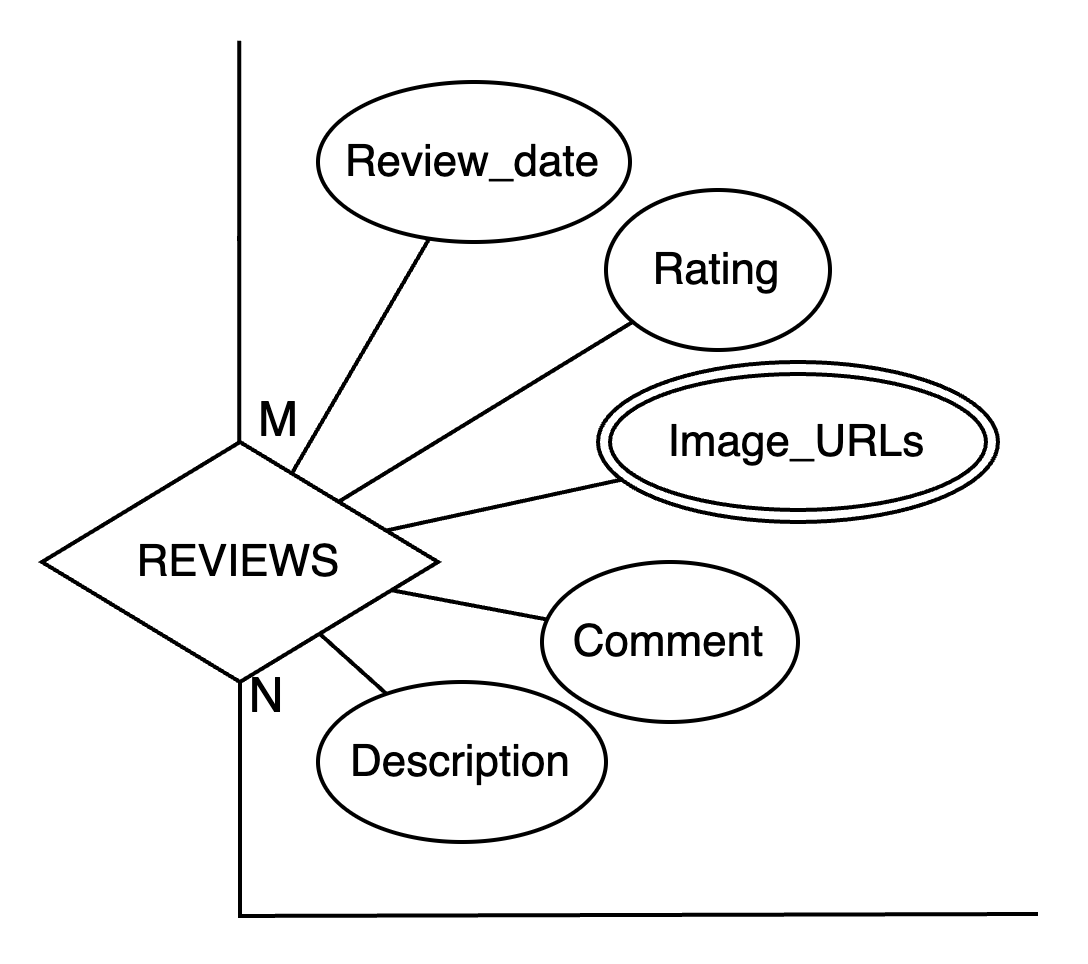
\includegraphics[width=0.7\textwidth]{images/relationships/reviews.png}
  \caption{\textit{Reviews Relationship}}
\end{figure}

The "Reviews" relationship connects the Customer and the Product. A customer can review several products, and a product can receive reviews from multiple customers. This helps gather feedback for product improvement.

\subsubsection{Subcategory}
\begin{figure}[H]
  \centering
  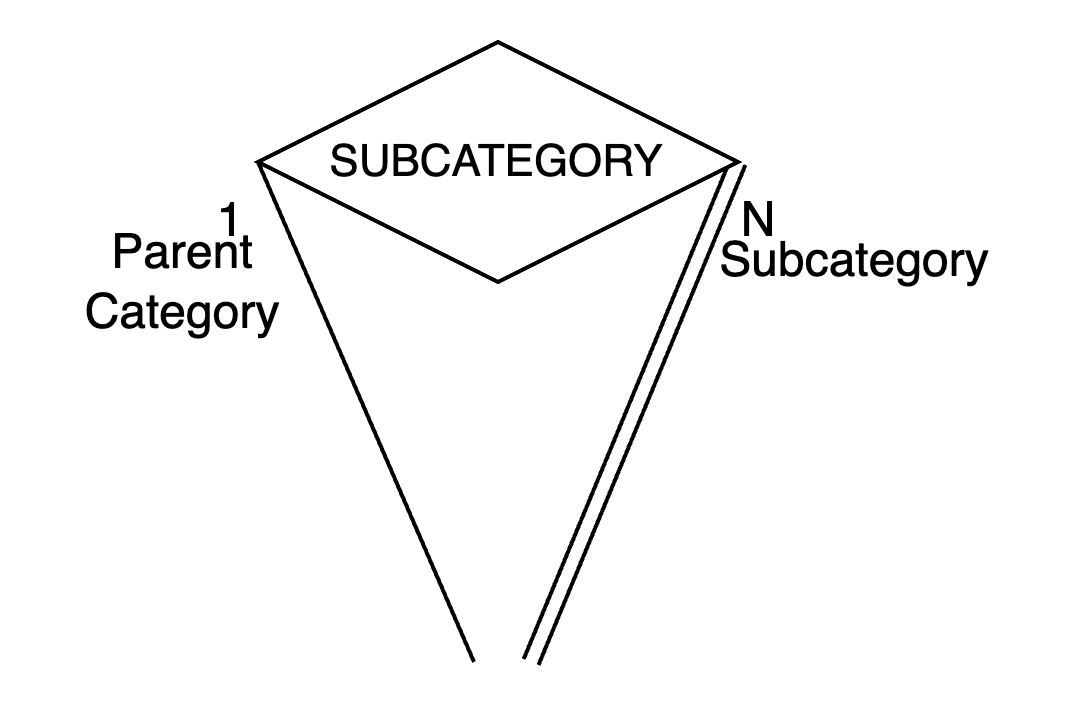
\includegraphics[width=0.7\textwidth]{images/relationships/subcategory.png}
  \caption{\textit{Subcategory Relationship}}
\end{figure}

The "Subcategory" relationship connects a Category to its subcategories. This relationship ensures hierarchical organization of product categories.

\subsubsection{Supply}
\begin{figure}[H]
  \centering
  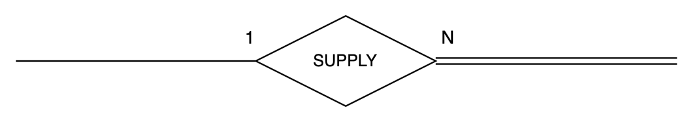
\includegraphics[width=0.7\textwidth]{images/relationships/supply.png}
  \caption{\textit{Supply Relationship}}
\end{figure}

The "Supply" relationship is between the Supplier and the Product. A supplier can supply multiple products. It tracks the quantity, date, and price of supplied products.

\subsubsection{Supervision}
\begin{figure}[H]
  \centering
  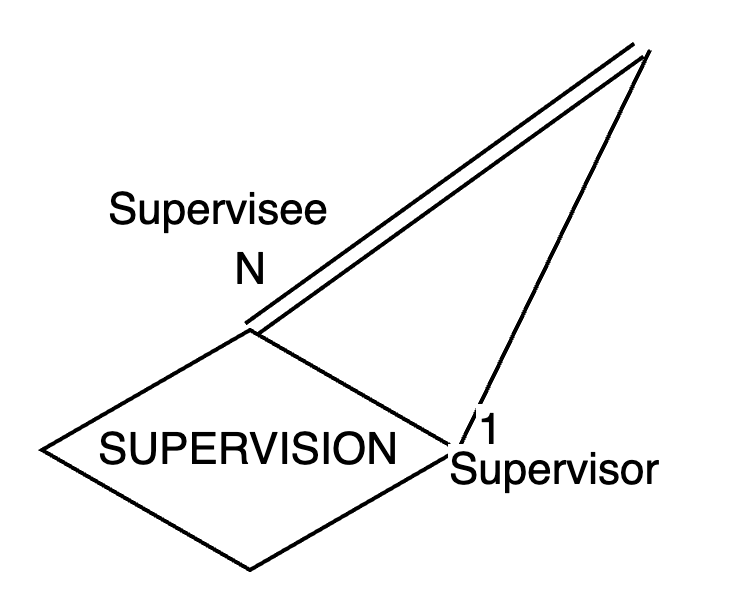
\includegraphics[width=0.7\textwidth]{images/relationships/supervision.png}
  \caption{\textit{Supervision Relationship}}
\end{figure}

The "Supervision" relationship is a recursive relationship among Employees. An employee can supervise others, ensuring a clear management hierarchy.

\subsubsection{Wishlist}
\begin{figure}[H]
  \centering
  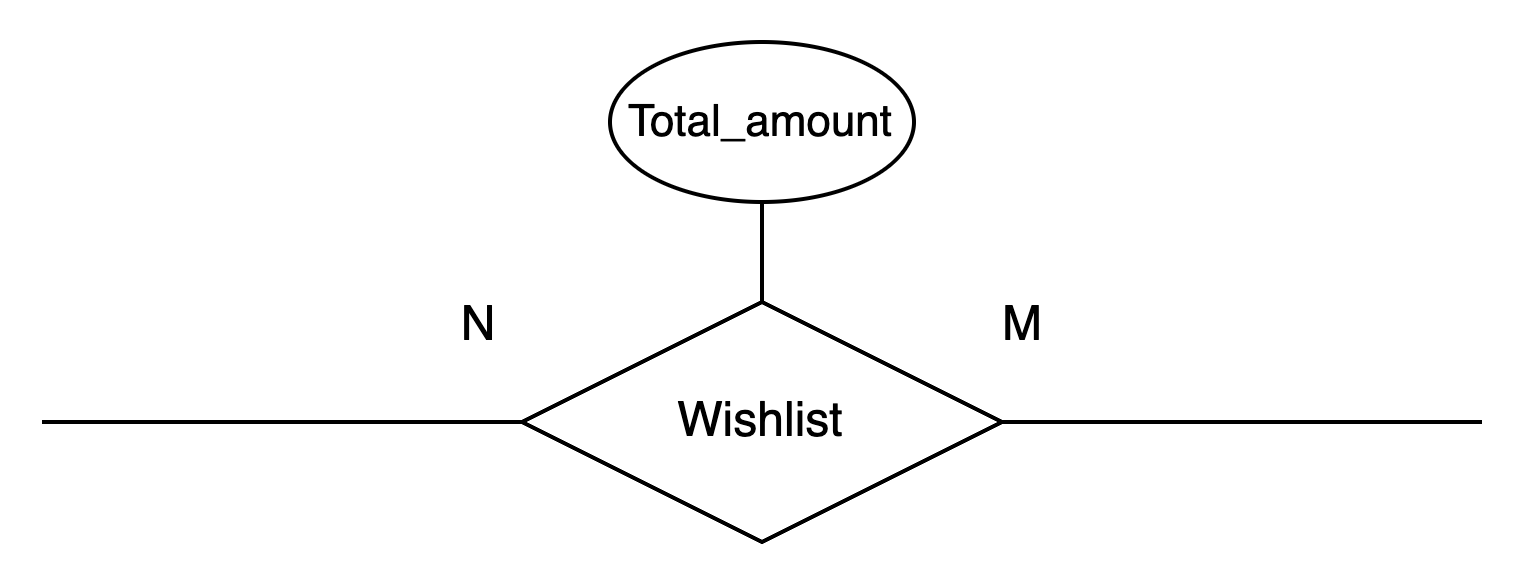
\includegraphics[width=0.7\textwidth]{images/relationships/wishlist.png}
  \caption{\textit{Wishlist Relationship}}
\end{figure}

The "Wishlist" relationship is between the customer and the product. A wishlist must be created by a customer. However, a wishlist can be empty, or it can include several products. It takes as an attribute the total amount (price) of the products. This relationship ensures that the customer can save the items he/she wishes to obtain later on.

\subsubsection{Works For}
\begin{figure}[H]
  \centering
  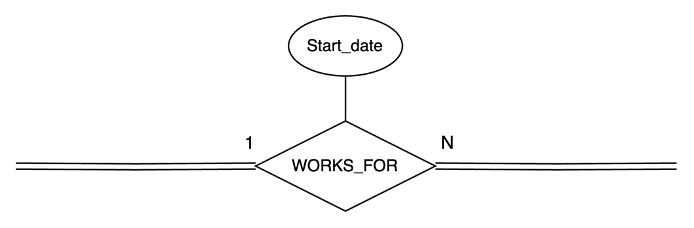
\includegraphics[width=0.7\textwidth]{images/relationships/works_for.png}
  \caption{\textit{Works For Relationship}}
\end{figure}

The "Works For" relationship connects the Employee and the Department. Many employees work for one department, and each department must have at least one employee.

\subsubsection{Works In}
\begin{figure}[H]
  \centering
  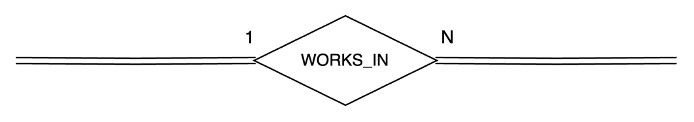
\includegraphics[width=0.7\textwidth]{images/relationships/works_in.png}
  \caption{\textit{Works In Relationship}}
\end{figure}

The "Works In" relationship links the Employee and the Branch. A branch must have at least one employee, and each employee works in one branch.